\documentclass[crop,tikz]{standalone}
\usepackage{tikz}
\usepackage{dsfont}
\usepackage{amsmath, amsthm, amssymb}
\usetikzlibrary{matrix, cd}
\usepackage{etoolbox}
\newcommand*\Z{\mathds{Z}}
\newcommand*\CP{\mathbb{CP}}
\newcommand*\ee[2]{H^{#1}(\CP^2) \otimes_{\Z} H^{#2}(S^1)}
\newcommand*\zt[2]{#1 \otimes_{\Z} #2}
\newcommand*\HT[2]{H^{#1}(\CP^2) \otimes_{\Z} #2}
\newcommand*\HCP[1]{H^{#1}(\CP^2)}


\newcommand\mygrid[3][]{      % this definition uses \foreach inside a matrix
  \let\mymatrixcontent\empty  % see http://tex.stackexchange.com/q/60394/18228
  \newcommand{\row}{%
    \foreach \j in {1,...,#2}{
      \foreach \i in {1,...,#3} {%
        \begingroup\edef\x{\endgroup
           \noexpand\gappto\noexpand\mymatrixcontent{|[draw,minimum size=1cm,#1]| \&}}\x
        }%
      \gappto\mymatrixcontent{\\}%
    }
  }
  \row
  \matrix(m)[matrix of nodes,ampersand replacement=\&,row sep=-\pgflinewidth,column sep=-\pgflinewidth]{
    \mymatrixcontent
  };
  \foreach \x[count=\i from 0] in {1,...,#2}\node[left] at (m-\x-1.west) {$\i$};
  \foreach \y[count=\j from 0] in {1,...,#3}\node[above] at (m-1-\y.north) {$\j$};
}





\newcommand*\ZZ{|[draw,circle]| \Z_2}
\usepackage{graphicx}
\usepackage{caption}

\begin{document}


% Writing All E2 terms
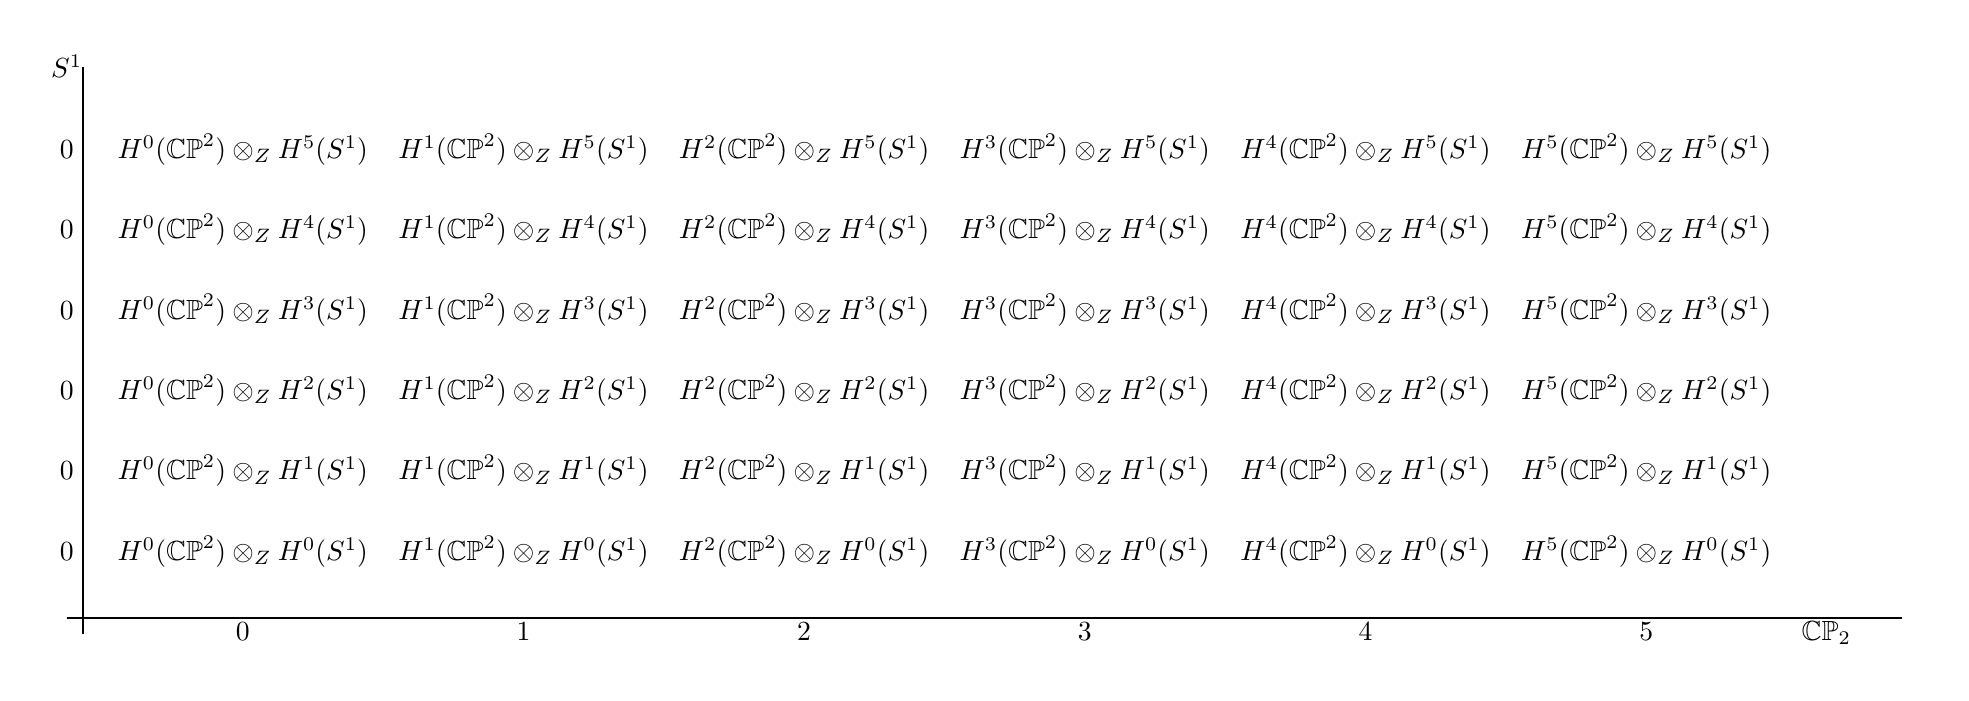
\begin{tikzpicture}
\matrix (m) [matrix of math nodes,
  nodes in empty cells,nodes={minimum width=5ex,
  minimum height=5ex,outer sep=-5pt},
  column sep=1ex,row sep=1ex]{
%
S^1& 	&   &  	& 	& 	&	&	&	\\
%
0&	\ee{0}{5}&	\ee{1}{5}&	\ee{2}{5}&	\ee{3}{5}&	\ee{4}{5}&	\ee{5}{5}&	&\\
0&	\ee{0}{4}&	\ee{1}{4}&	\ee{2}{4}&	\ee{3}{4}&	\ee{4}{4}&	\ee{5}{4}&	&\\
0&	\ee{0}{3}&	\ee{1}{3}&	\ee{2}{3}&	\ee{3}{3}&	\ee{4}{3}&	\ee{5}{3}&	&\\
0&	\ee{0}{2}&	\ee{1}{2}&	\ee{2}{2}&	\ee{3}{2}&	\ee{4}{2}&	\ee{5}{2}&	&\\
0&	\ee{0}{1}&	\ee{1}{1}&	\ee{2}{1}&	\ee{3}{1}&	\ee{4}{1}&	\ee{5}{1}&	&\\
0&	\ee{0}{0}&	\ee{1}{0}&	\ee{2}{0}&	\ee{3}{0}&	\ee{4}{0}&	\ee{5}{0}&	&\\ \quad\strut
%
&	0&	1&	2&	3&	4&	5&	\CP_2& \strut \\};
%
\draw[thick] (m-8-1.east) -- (m-1-1.east) ;
\draw[thick] (m-8-1.north) -- (m-8-9.north) ;
\end{tikzpicture}

\vspace{1cm}

% Plugging in known groups
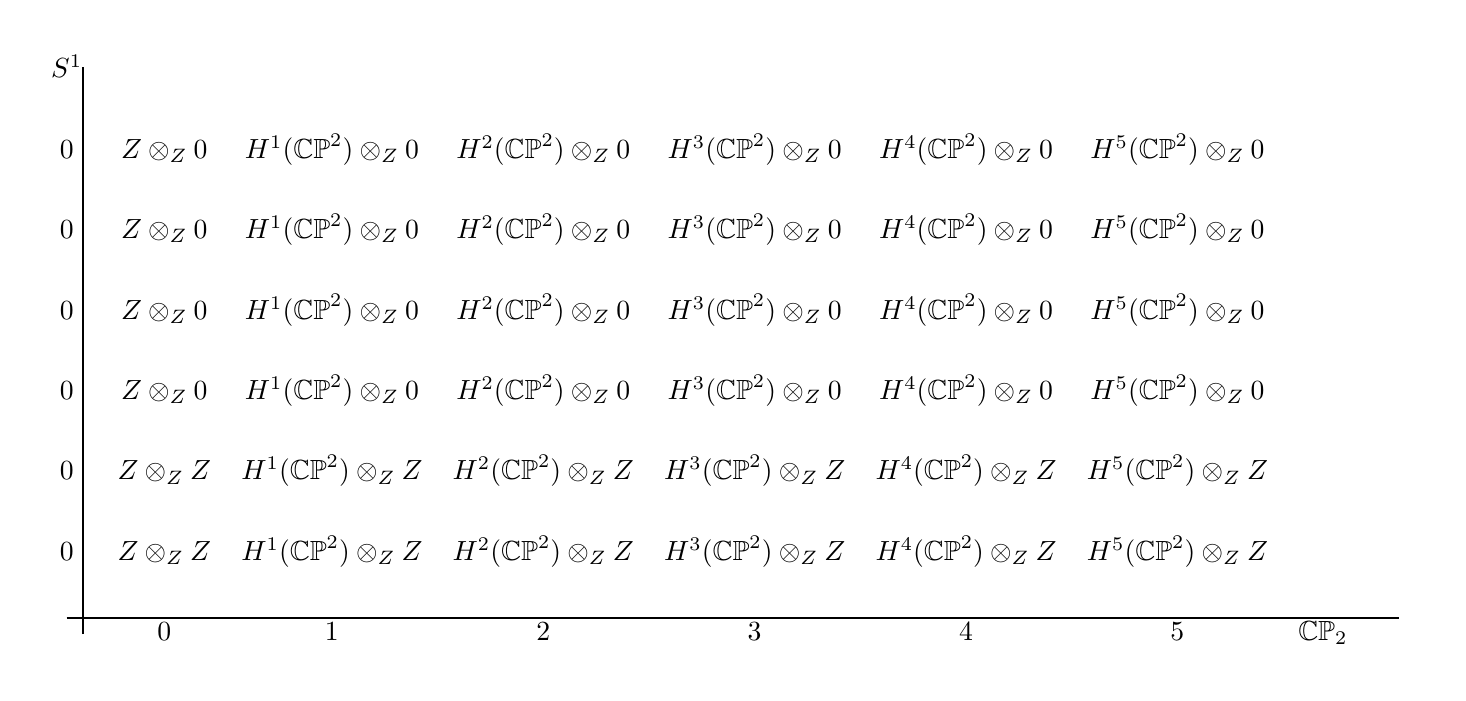
\begin{tikzpicture}
\matrix (m) [matrix of math nodes,
  nodes in empty cells,nodes={minimum width=5ex,
  minimum height=5ex,outer sep=-5pt},
  column sep=1ex,row sep=1ex]{
%
S^1& 	&   &  	& 	& 	&	&	&	\\
%
0&	\zt{\Z}{0}&		\HT{1}{0}&	\HT{2}{0}&	\HT{3}{0}&	\HT{4}{0}&	\HT{5}{0}&	&\\
0&	\zt{\Z}{0}&		\HT{1}{0}&	\HT{2}{0}&	\HT{3}{0}&	\HT{4}{0}&	\HT{5}{0}&	&\\
0&	\zt{\Z}{0}&		\HT{1}{0}&	\HT{2}{0}&	\HT{3}{0}&	\HT{4}{0}&	\HT{5}{0}&	&\\
0&	\zt{\Z}{0}&		\HT{1}{0}&	\HT{2}{0}&	\HT{3}{0}&	\HT{4}{0}&	\HT{5}{0}&	&\\
0&	\zt{\Z}{\Z}&	\HT{1}{\Z}&	\HT{2}{\Z}&	\HT{3}{\Z}&	\HT{4}{\Z}&	\HT{5}{\Z}&	&\\
0&	\zt{\Z}{\Z}&	\HT{1}{\Z}&	\HT{2}{\Z}&	\HT{3}{\Z}&	\HT{4}{\Z}&	\HT{5}{\Z}&	&\\ \quad\strut
%
&	0&	1&	2&	3&	4&	5&	\CP_2& \strut \\};
%
\draw[thick] (m-8-1.east) -- (m-1-1.east) ;
\draw[thick] (m-8-1.north) -- (m-8-9.north) ;
\end{tikzpicture}

% Simplifying
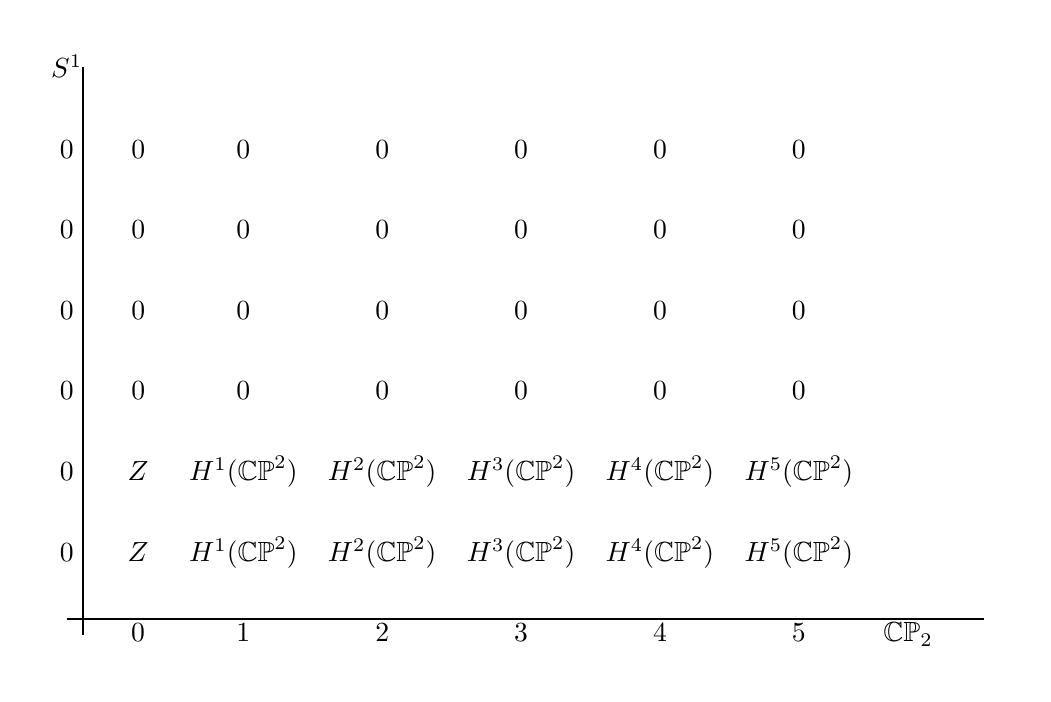
\begin{tikzpicture}
\matrix (m) [matrix of math nodes,
  nodes in empty cells,nodes={minimum width=5ex,
  minimum height=5ex,outer sep=-5pt},
  column sep=1ex,row sep=1ex]{
%
S^1& 	&   &  	& 	& 	&	&	&	\\
%
0&	0&		0&	0&	0&	0&	0&	&\\
0&	0&		0&	0&	0&	0&	0&	&\\
0&	0&		0&	0&	0&	0&	0&	&\\
0&	0&		0&	0&	0&	0&	0&	&\\
0&	\Z&	\HCP{1}&	\HCP{2}&	\HCP{3}&	\HCP{4}&	\HCP{5}&	&\\
0&	\Z&	\HCP{1}&	\HCP{2}&	\HCP{3}&	\HCP{4}&	\HCP{5}&	&\\ \quad\strut
%
&	0&	1&	2&	3&	4&	5&	\CP_2& \strut \\};
%
\draw[thick] (m-8-1.east) -- (m-1-1.east) ;
\draw[thick] (m-8-1.north) -- (m-8-9.north) ;
\end{tikzpicture}

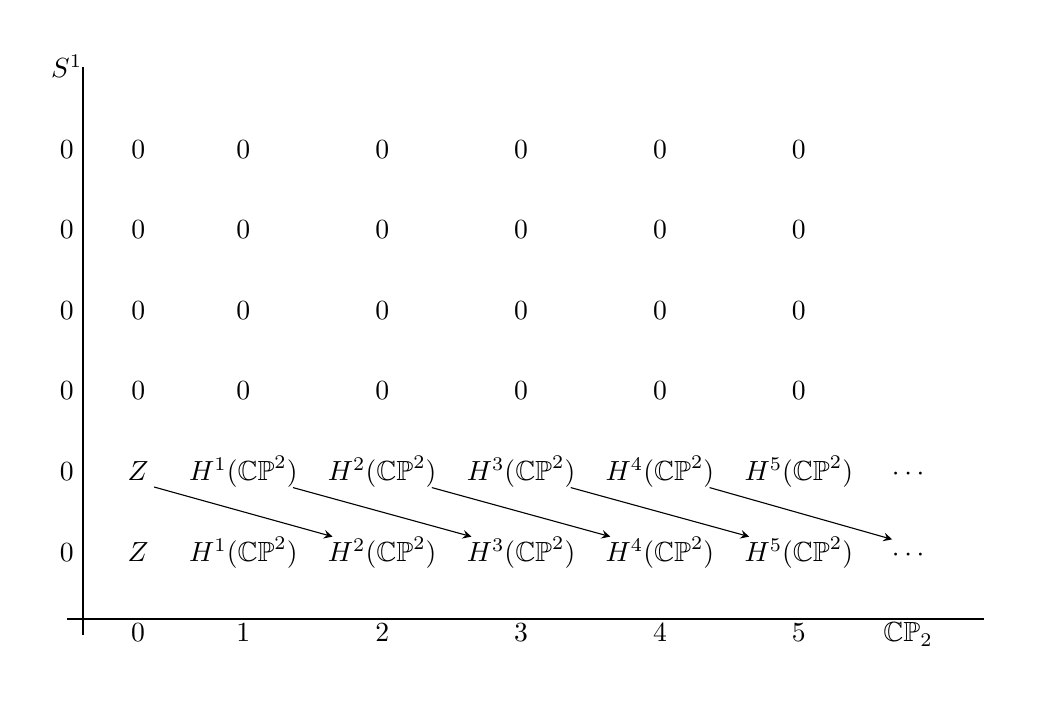
\begin{tikzpicture}
\matrix (m) [matrix of math nodes,
  nodes in empty cells,nodes={minimum width=5ex,
  minimum height=5ex,outer sep=-5pt},
  column sep=1ex,row sep=1ex]{
%
S^1& 	&   &  	& 	& 	&	&	&	\\
%
0&	0&		0&	0&	0&	0&	0&	&\\
0&	0&		0&	0&	0&	0&	0&	&\\
0&	0&		0&	0&	0&	0&	0&	&\\
0&	0&		0&	0&	0&	0&	0&	&\\
0&	\Z&	\HCP{1}&	\HCP{2}&	\HCP{3}&	\HCP{4}&	\HCP{5}&	\cdots&\\
0&	\Z&	\HCP{1}&	\HCP{2}&	\HCP{3}&	\HCP{4}&	\HCP{5}&	\cdots&\\ \quad\strut
%
&	0&	1&	2&	3&	4&	5&	\CP_2& \strut \\};
%
\draw[thick] (m-8-1.east) -- (m-1-1.east) ;
\draw[thick] (m-8-1.north) -- (m-8-9.north) ;
\draw[-stealth] (m-6-2.south east) -- (m-7-4.north west);
\draw[-stealth] (m-6-3.south east) -- (m-7-5.north west);
\draw[-stealth] (m-6-4.south east) -- (m-7-6.north west);
\draw[-stealth] (m-6-5.south east) -- (m-7-7.north west);
\draw[-stealth] (m-6-6.south east) -- (m-7-8.north west);

\end{tikzpicture}

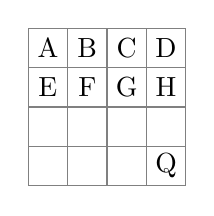
\begin{tikzpicture}
\draw[step=0.5cm,color=gray] (-1,-1) grid (1,1);
\node at (-0.75,+0.75) {A};
\node at (-0.25,+0.75) {B};
\node at (+0.25,+0.75) {C};
\node at (+0.75,+0.75) {D};
\node at (-0.75,+0.25) {E};
\node at (-0.25,+0.25) {F};
\node at (+0.25,+0.25) {G};
\node at (+0.75,+0.25) {H};
% ...
\node at (+0.75,-0.75) {Q};
\end{tikzpicture}

\tikz\draw grid(4,4)foreach[count=~]\l in{1,...,16}{
({.5+mod(~-1,4},{3.5-div(~-1,4})node{$H^1 \mathbb{CP}^\l$}
};


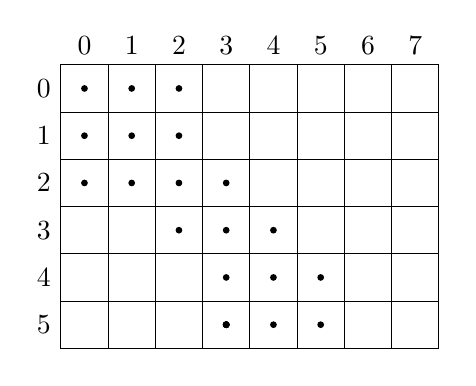
\begin{tikzpicture}[scale=.5,]
\mygrid[scale=.6]{6}{8} % two extra columns just for demonstration

\foreach\j[count=\i,remember=\i as \x(initially 3)] in{1,...,6}{
  \filldraw(m-\i-\j)circle[radius=2pt];
  \filldraw(m-\x-\j)circle[radius=2pt];
  \filldraw(m-\j-\x)circle[radius=2pt];
  \filldraw(m-6-4)circle[radius=2pt];
}
\end{tikzpicture}

\begin{tikzcd}
 &  &  &  & 0 \arrow[lllldd] \\
 &  &  &  &  \\
H_2S^1 \arrow[rr] \arrow[rr, "{(i^*, -j^*)}"] &  & H_2 M \oplus H_2 D^2 \arrow[rr, "l^* - r^*"] &  & H_2 \mathbb{RP}^2 \arrow[lllldd, "\delta_2"'] \\
 &  &  &  &  \\
H_1S^1 \arrow[rr, "{(i^*, -j^*)}"] &  & H_1 M \oplus H_1 D^2 \arrow[rr, "l^*-r^*"] &  & H_1 \mathbb{RP}^2 \arrow[lllldd, "\delta_1"'] \\
 &  &  &  &  \\
H_0 S^1 \arrow[rr, "{(i^*, -j^*)_0}"] &  & H_0 M \oplus H_0 D^2 \arrow[rr, "(l^* - r^*)_0"] &  & H_0 \mathbb{RP}^2 \arrow[lllldd, "\delta_0"] \\
 &  &  &  &  \\
0 &  &  &  &
\end{tikzcd}


\begin{tikzcd}
 &  &  &  & 0 \arrow[lllldd, out=0, in=-180, "0"'] \\
 &  &  &  &  \\
0 \arrow[rr] \arrow[rr, "{(0, 0)}"] &  & 0 \oplus 0 \arrow[rr, "0"] &  & \delta M\mathbb{RP}^2 \arrow[lllldd, "\delta_2"', out=0, in=-180] \\
 &  &  &  &  \\
\mathbb{Z} \arrow[rr, "{x\mapsto (2x, 0)}"] &  & \mathbb{Z} \oplus 0 \arrow[rr, "{(x,0) \mapsto x}"] &  & H_1 \mathbb{RP}^2 \arrow[lllldd, "\delta_1"', out=0, in=-180] \\
 &  &  &  &  \\
\mathbb{Z} \arrow[rr, "{(i^0, -j^0)}"] &  & \mathbb{Z} \oplus \mathbb{Z} \arrow[rr, "l^0 - r^0"] &  & H_0 \mathbb{RP}^2 \arrow[lllldd, "\delta_0"', out=0, in=-180] \\
 &  &  &  &  \\
0 &  &  &  &
\end{tikzcd}



\end{document}
